	% 代码分析:模块功能、涉及到的类、类关系、数据结构及关键代码等;
	% 任务要求,设计任务要求;
	% 设计:详细的设计方案,相关的数据结构、算法描述,可采用伪代码等形式化描述
	% 实现:修改哪些类、如何修改、为什么修改等;
	% 测试:测试用例,测试结果及结果分析,测试运行界面等;
	% 调试:调试方法,遇到的问题及解决方案等;
	% 结论与展望:完成的主要工作、收获、进一步的工作,建议、体会、心得等;

\section{作业8}
\subsection{作业8.1}
\subsubsection{题目描述}
\begin{figure}[H]
    \centering
    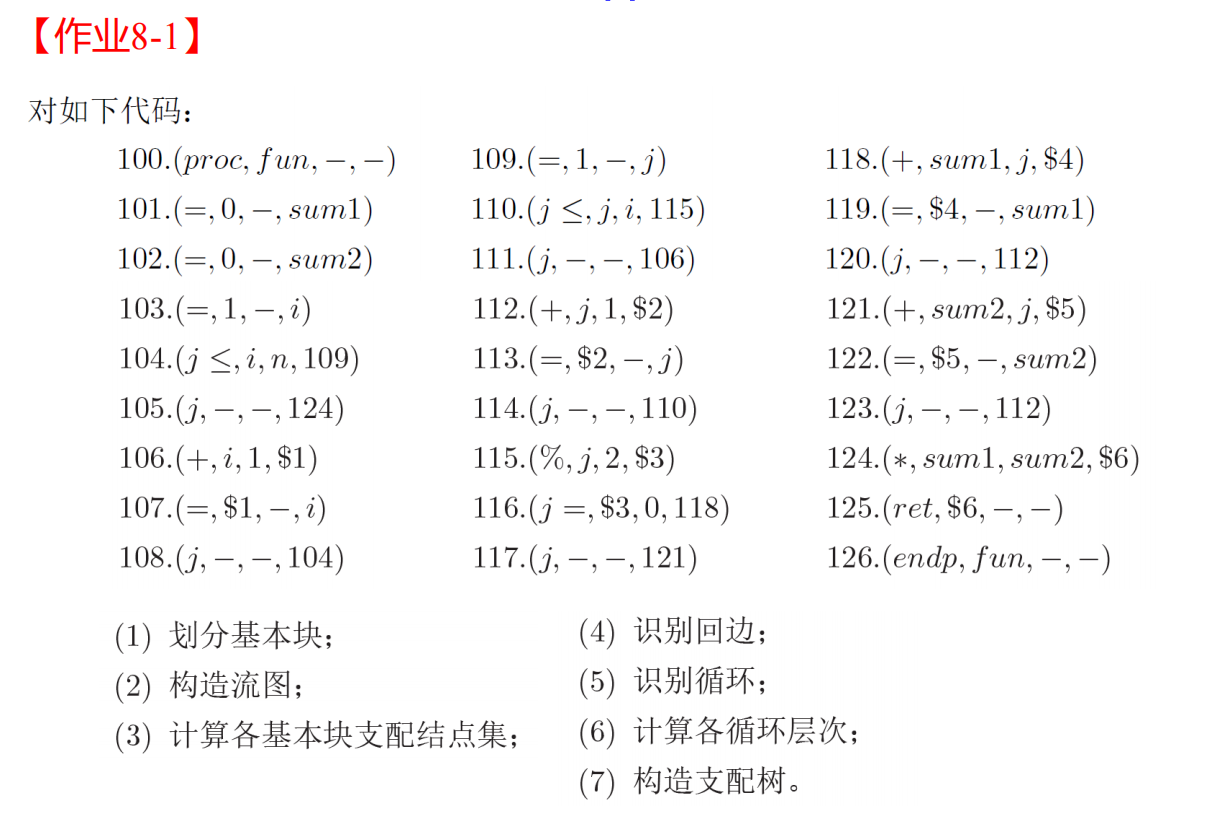
\includegraphics[width=0.9\linewidth]{imgs/8_1.png}
    \caption{作业 8.1——题目}
    \label{fig:8_1_prob}
\end{figure}
\subsubsection{解答}

求出基本块入口:

\begin{figure}[H]
    \centering
    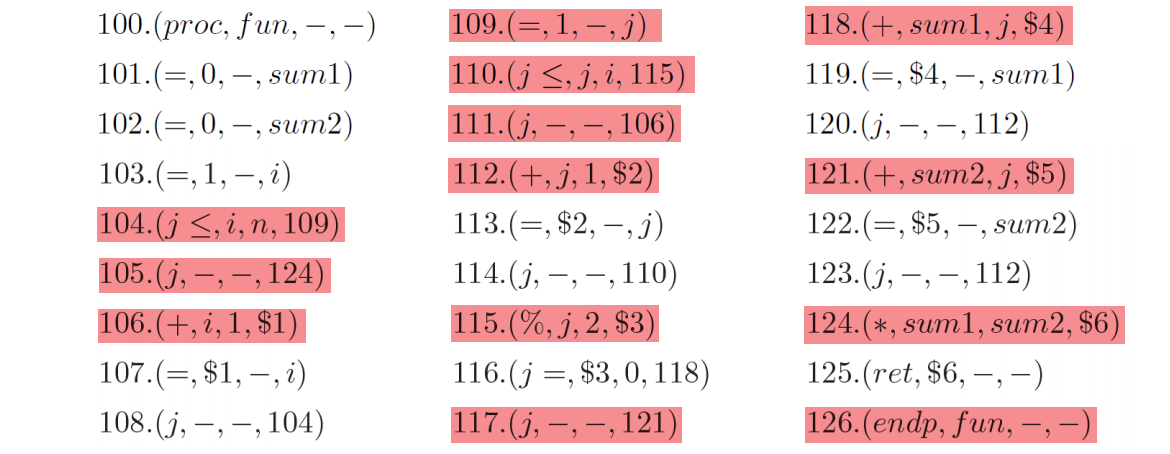
\includegraphics[width=0.9\linewidth]{imgs/8_1_1.png}
    \caption{作业 8.1——基本块入口}
    \label{fig:8_1_prob}
\end{figure}

划分基本块:

\begin{figure}[H]
    \centering
    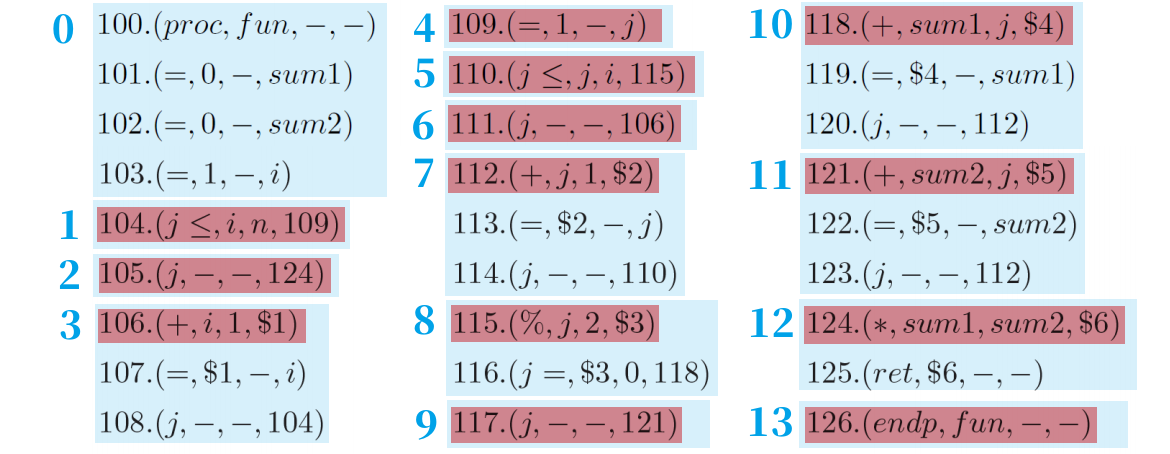
\includegraphics[width=0.9\linewidth]{imgs/8_1_2.png}
    \caption{作业 8.1——基本块}
    \label{fig:8_1_prob}
\end{figure}

构造流图:

\begin{center}
\begin{tikzpicture}[node distance=0.5cm, auto]
    \tikzstyle{block} = [rectangle, draw, fill=white!20, 
    text width=3em, text centered, rounded corners, minimum height=1.6em]

    \node [block] (B1) {$\text B_0$};
    \node [block, below=of B1] (B2) {$\text B_1$};
    \node [block, below=of B2] (B3) {$\text B_2$};
    \node [block, below=of B3] (B13) {$\text B_{12}$};
    \node [block, below=of B13] (B14) {$\text B_{13}$};

    \node [block, right=2cm of B2] (B5) {$\text B_4$};
    \node [block, below=of B5] (B6) {$\text B_5$};
    \node [block, below=of B6] (B7) {$\text B_6$};
    \node [block, below=of B7] (B4) {$\text B_3$};

    \node [block, right=2cm of B6] (B9) {$\text B_8$};
    \node [block, below=of B9] (B10) {$\text B_9$};
    \node [block, below=of B10] (B12) {$\text B_{11}$};
    \node [block, below=of B12] (B8) {$\text B_7$};

    \node [block, right=2cm of B9] (B11) {$\text B_{10}$};

    \draw [->] (B1) -- (B2);
    \draw [->] (B2) -- (B3);
    \draw [->] (B3) -- (B13);
    \draw [->] (B13) -- (B14);

    \draw [->] (B2) -- (B5);
    \draw [->] (B5) -- (B6);
    \draw [->] (B6) -- (B7);
    \draw [->] (B7) -- (B4);

    \draw [->] (B6) -- (B9);
    \draw [->] (B9) -- (B10);
    \draw [->] (B10) -- (B12);
    \draw [->] (B12) -- (B8);

    \draw [->] (B9) -- (B11);
    \draw [->] (B11) -- (B8);

    \draw [->] (B4) -- (B2);
    \draw [->] (B8) -- (B6);
    \draw [->] (B11) -- (B8);
\end{tikzpicture}
\end{center}

\subsection{作业8.2}
\subsubsection{题目描述}
\begin{figure}[H]
    \centering
    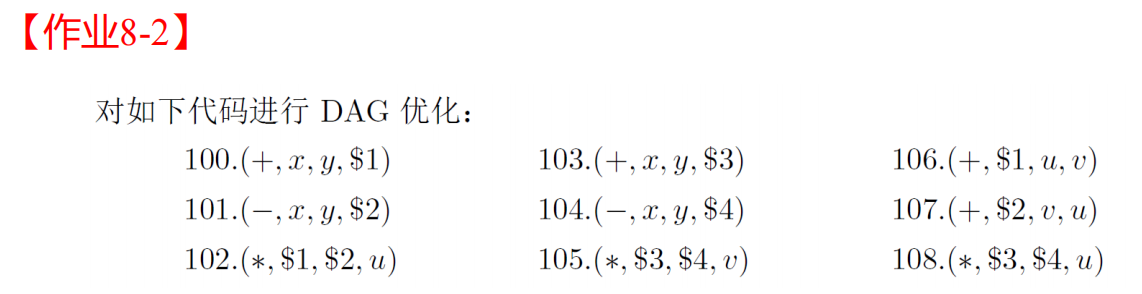
\includegraphics[width=0.9\linewidth]{imgs/8_2.png}
    \caption{作业 8.2——题目}
    \label{fig:8_2_prob}
\end{figure}
\subsubsection{解答}

使用 DAG 优化:

\begin{table}[H]
    \centering
    \begin{tabular}{c|c}
        \begin{tikzpicture}[node distance=0.8cm, auto, baseline=(current bounding box.center)]
    \tikzstyle{block} = [circle, draw, fill=white!20, 
    text width=1em, text centered, rounded corners, minimum height=1em]

    \node [block, label={left:$v$}] (v) {$+$};
    \node [block, below right=0.8cm and 0.4cm of v, label={right:$u$}] (u) {$*$};
    \node [block, below=of u, label={right:\$1,\$3}] (plus) {$+$};
    \node [block, left=of plus, label={left:\$2,\$4}] (minus) {$-$};
    \node [block, below=of minus] (x) {$x$};
    \node [block, below=of plus] (y) {$y$};

    \draw [-] (v) -- node[auto] {} (u);
    \draw [-] (v) -- node[auto] {} (minus);
    \draw [-] (u) -- node[auto] {} (plus);
    \draw [-] (u) -- node[auto] {} (minus);
    \draw [-] (x) -- node[auto] {} (plus);
    \draw [-] (y) -- node[auto] {} (plus);
    \draw [-] (y) -- node[auto] {} (minus);
    \draw [-] (x) -- node[auto] {} (minus);
\end{tikzpicture}
        &
            \begin{tabular}{ll}
              100. & $(+,x,y,\$1)$ \\
              101. & $(=,\$1,-,\$3)$ \\
              102. & $(-,x,y,\$2)$ \\
              103. & $(=,\$2,-,\$4)$ \\
              104. & $(*,\$1,\$2,u)$ \\
              105. & $(+,\$1,u,v)$ \\
            \end{tabular}
        \\
    \end{tabular}
\end{table}
